
\chapter {Policy}

La Policy sulla Sicurezza Informatica è quel documento nel quale sono
contenute tutte le
disposizioni, comportamenti e misure organizzative richieste ai dipendenti
e/o collaboratori
aziendali per contrastare i rischi informatici. Si va a identificare tutte
quelle regole che possono
essere stabilite su un Server così che le workstation collegate vengano
"controllate" nella stessa
maniera e per fare in modo che su di esse siano presenti le stesse
caratteristiche.
L’obiettivo è quello di garantire i tre goal della Sicurezza:
confidenzialità, integrità e disponibilità.
Il compito della policy è quello di stabilire cosa è permesso e cosa non
lo è, cioè distinguere cosa è
reputato sicuro (e quindi autorizzato) da cosa invece può portare ad una
violazione del sistema. Il
sistema si muove da uno stato ad un altro. Ciò che deve fare la policy è
fare in modo che questo
non assuma mai in stati non sicuri. Un sistema si dice “sicuro” quando ciò
non accade mai.
Quando un sistema permette ad un utente o ad un processo di entrare in uno
stato non autorizzato
si dice che si è verificato un “security breach”.
Sia X un set di entità e I un informazione:
\begin{itemize}
      \item I ha confidenzialità con rispetto a X se nessun membro di X può
            ottenere alcuna
            informazione su I;
      \item I ha integrità con rispetto a X se tutti i membri di X si fidano
            di I. Le nozioni di “fiducia” e
            “integrità” sono collegate. Se un sistema ha integrità, dobbiamo
            fidarci del fatto che il suo
            comportamento è corretto. Se I è una risorsa, la sua integrità implica
            che essa funzioni
            come dovrebbe (assurance);
      \item I ha disponibilità con rispetto a X se tutti i membri di X hanno
            accesso ad I.
\end{itemize}


\paragraph{Confidentiality Policy.}

Il suo scopo è garantire che tutto lo staff comprenda i requisiti
dell'organizzazione in relazione alla
divulgazione di dati personali e informazioni riservate.
Riguardo al flusso delle informazioni è possibile possedere diversi
diritti. Si può, infatti:
\begin{itemize}
      \item Trasferire i diritti di accesso;
      \item Trasferire le informazioni senza però trasferire i diritti;
      \item Avere diritto di accesso alle informazioni solo per un certo
            periodo di tempo.
\end{itemize}

Il modello della policy spesso dipende dalla fiducia.

\paragraph{Integrity Policy.}

Definisce come l’informazione può essere modificata o alterata.
Specifica:
\begin{itemize}
      \item Chi può effettivamente compiere queste operazioni;
      \item Sotto quali condizioni i dati possono essere alterati;
      \item Eventuali limiti sulle modifiche dei dati.
\end{itemize}

Un mezzo per ottenere l’integrità è la separazione dei compiti.
Si deve fare in modo che tutte le operazioni compiute (transazioni) mantengano il sistema in uno
stato “consistente”.

\paragraph{Availability.}

Tipi di disponibilità:
\begin{itemize}
      \item Tradizionale: x ha o no l’accesso;
      \item Quality of Service: viene promesso un certo livello di accesso
            che però non è garantito (ad esempio, un livello
            specifico di larghezza di banda).
\end{itemize}

\paragraph{La policy e i suoi meccanismi: }
La policy descrive ciò che è permesso e cosa no, i meccanismi,
invece, controllano come questa viene implementata. Chiaramente gli utenti devono verificarsi
della policy, ma anche dei meccanismi utilizzati.
Le policy prese in considerazione per il controllo sugli accessi sono:
\begin{itemize}
      \item Discretionary Access Control (DAC): il proprietario determina i diritti di accesso.
            Solitamente sono identity-based access control (IBAC), ovvero il proprietario indica anche
            quali altri utenti possono avere l’accesso;
      \item Mandatory Access Control (MAC): policy più restrittive. Stabiliscono a priori quali sono i
            comportamenti da evitare e quelli permessi. Ciò non viene specificato da chi crea la risorse,
            ma anche dalle regole generali che vengono messe in atto, per esempio quelle aziendali;
      \item Originator Controlled Access Control (ORCON): policy dove colui che assegna i diritti è il
            creatore. I possessori dei file non detengono diritti e non possono cederli a loro volta;
      \item Role Based Access Control (RBAC): usate in ambito commerciale per la gestione delle
            risorse a livello amministrativo e aziendale.
            Quando si definisce una policy si devono sempre tenere presenti:
      \item Gli utenti;
      \item I ruoli che essi ricoprono: utente, utente segreto, sistemista, utente negligente..
      \item Le operazioni che possono essere compiute o no: leggere, scrivere, “downgrade”, cambio
            password...
      \item Le modalità con cui vietare o consentire determinate operazioni: obbligo, permesso, divieto,
            discrezionalità..
\end{itemize}

\section{Confidentiality Policies}
Una politica di riservatezza, chiamata anche “information flow policy”, 
impedisce la divulgazione
non autorizzata di informazioni. Il suo obiettivo è quello di specificare quali 
dati devono essere
protetti e da chi o da che cosa vanno protetti. In poche parole, indicano un 
insieme di principi e
regole che definiscono i possibili accessi al sistema.

Distinguiamo tra:

\begin{itemize}
      \item \textbf{Oggetti:} una qualunque entità passiva che necessita di
            essere protetta;
      \item \textbf{Soggetti:} una qualunque entità attiva che può manipolare
            gli oggetti (persone o processi).
\end{itemize}

Un modello di sicurezza definisce i soggetti, gli oggetti ai quali i soggetti 
hanno accesso ed i diritti
di accesso, che non sono altro che le operazioni con le quali è possibile 
operare. Un soggetto può
avere diritti di accesso sia per gli oggetti che per altri soggetti.
Esistono due tipi di modelli di sicurezza:
\begin{itemize}
      \item \textit{Discretionary access control} (\textbf{DAC}): meccanismo
            attraverso il quale gli utenti possono
            liberamente decidere di garantire o revocare l’accesso a determinati
            oggetti.
            \begin{itemize}
                  \item Gli utenti amministrano i dati che possiedono (vengono
                        detti proprietari);
                  \item Il proprietario può autorizzare altri utenti all’accesso;
                  \item Il proprietario può definire il tipo di accesso da
                        concedere agli altri;
                  \item Accessi selettivi.
            \end{itemize}
      \item \textit{Mandatory access control} (\textbf{MAC}): meccanismo
            attraverso il quale le decisioni di accesso
            sono basate su delle etichette che contengono informazioni 
            rilevanti alla sicurezza di un
            oggetto. Questo metodo fornisce l'accesso alla risorsa in base al
            livello di autorizzazione dell'utente.
            \begin{itemize}
                  \item Classificazione dei dati (livelli di sensibilità);
                  \item Classificazione dei soggetti (autorizzazione);
                  \item Classe di sicurezza <componente gerarchica, insiemi di
                        categoria>;
                  \item Ordinamento (parziale) tra le classi di sicurezza;
                  \item I meccanismi di sicurezza devono garantire che tutti i
                        soggetti abbiano accesso solo
                        ai dati per cui possiedono le autorizzazioni appropriate;
                  \item Non si possono propagare privilegi.
            \end{itemize}
\end{itemize}

\subsection{Modello Bell-LaPadula}
\'{E} un modello tipico MAC. Fu proposto da Bell-LaPadula nel 1976 con lo scopo di 
rafforzare i
controlli ai possibili accessi alle applicazioni militari (corrisponde, infatti, 
alle classificazioni
stile-militare). Viene anche chiamato modello “a multi-livelli”.
Nelle applicazioni i soggetti e gli oggetti vengono partizionati in differenti 
livelli di sicurezza. Un
soggetto può solo accedere ad oggetti a certi livelli, i quali sono dipendono 
strettamente dal loro
livello di sicurezza. Per esempio, i seguenti sono due tipici specificazioni di 
accessi: “una persona
UNCLASSIFIED non può leggere informazioni a livello CONFIDENTIAL” e 
“informazioni TOP
SECRET non possono essere scritte in files di livello UNCLASSIFIED”.
Gli oggetti sono classificati in 4 diversi livelli di sensibilità, cioè di 
confidentiality. Ciascun oggetto
può essere associato a uno o più livelli, detti compartments.
Ad ogni soggetto, invece, viene associata una “clearance” ovvero 
un’autorizzazione. Una
clearance non è altro che una coppia del tipo <rank, compartments> dove Rank è 
il massimo
livello di sensibilità dell’informazione a cui il soggetto ha accesso; 
Compartment indica i comparti a
cui il soggetto può accedere.
A tutte le entità vengono assegnati dei livelli di sicurezza. In particolare:

\begin{itemize}
      \item Un soggetto S possiede “security clearance” \(L(S)=l_s\);
      \item Un oggetto O possiede “security classification” \(L(O)=l_o\);
\end{itemize}

Per ogni classificazione di sicurezza \(l_i, \ i=0,...,k-1 \ con \ l_i<l_i+1\), 
quindi i livelli di sicurezza sono
disposti in ordine lineare.
Il tipo più semplice di classificazione della confidenzialità è un insieme di 
autorizzazioni poste in
gerarchia: Top secret > Secret > Confidential > Unclassified.
Il modello definisce due regole obbligatorie del controllo accessi (MAC):
\begin{itemize}
      \item \textbf{Simple Security Condition:} S può leggere O se e solo se
            \(l_o \le l_s\) e S ha discrezione
            nell’accesso in lettura a O. Questa regola viene anche detta “No Read Up” 
            e impedisce ai
            soggetti di leggere oggetti a livelli superiori. Il proprietario può 
            aggiungere anche dei diritti di
            tipo DAC, ovvero può restringere ulteriormente l’accesso.
      \item \textbf{* Property} (Star property): S può scrivere su O se e solo
            se \(l_s \le l_o\) e S ha discrezione
            nell’accesso alla scrittura su O. La regola è anche detta “No Write Down” 
            e impedisce ai
            soggetti di scrivere su oggetti di livello inferiore. Questo perché se no 
            un utente potrebbe declassificare 
            informazioni o oggetti scrivendoli all'interno di oggetti con grado di 
            classificazione inferiore.
\end{itemize}

Si potrebbe estendere il modello addizionando un gruppo di categorie per ogni 
classificazione di
sicurezza. Ogni categoria descrive un tipo di informazioni.
Tali categorie risultano dal principio del “Need To know”: limito l’accesso alle
sole informazioni per
le quali l’utente ha necessità di accedere.

\paragraph{Esempio:}
CATEGORIE \(\rightarrow\) NUC, EUR e US
Ogni soggetto ha un’autorizzazione ad un determinato livello di sicurezza e può 
accedere anche
ad alcuni dei livelli inferiori.

\begin{figure}[H]
      \centering
      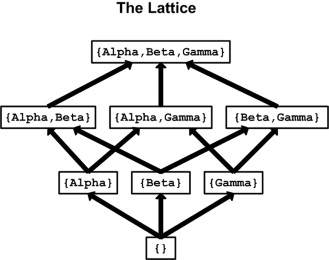
\includegraphics[width=8cm, keepaspectratio]{capitoli/policy/imgs/Lattuce.jpg}
\end{figure}

\subsection{Multilevel Security}
Il concetto viene trattato per la prima volta nel “Red Book”nel 1987.
La sicurezza multilivello o più livelli di sicurezza (\textbf{MLS}) è 
l'applicazione di un sistema di computer
per elaborare le informazioni con incompatibili classificazioni (cioè, a diversi 
livelli di sicurezza),
consentire l'accesso da parte di utenti con diversi spazi di sicurezza e le 
esigenze di sapere (need
to know) e impedire agli utenti di ottenere l'accesso alle informazioni per 
le quali non hanno
l'autorizzazione.
La sicurezza multilivello viene implementata in ambiti particolari, dove è 
necessario un controllo
obbligatorio degli accessi, per assicurare che le politiche di sicurezza siano 
garantite dal sistema.
L'ente definisce delle regole in merito a chi può accedere e anche a che cosa; 
queste regole non
possono essere modificate dai singoli utenti.
I sistemi MLS ci assicurano diversi livelli di sicurezza L che definiscono la 
classificazione dei
soggetti (processi) e degli oggetti. I livelli di affidabilità, cioè di 
“assurance”, vengono stabiliti in
base a vari criteri di valutazione:
\[
      (worst) \ D<C1<C2<C3<B1<B2<B3<A1 \ (best)
\]
In base ai dati e alle circostanze possono essere richiesti livelli più o meno 
elevati. Solitamente, in
presenza di un solo livello, è sufficiente una macchina del tipo C2 o C3. Da B1 
in poi, invece, si
possono gestire efficacemente informazioni su livelli multipli.
\begin{center}
      \begin{tabular}{ |c|c| }
            \hline
            \textbf{System Stores}   & \textbf{Minimum Assurance} \\
            \hline
            TopSecret + Unclassified & B3                         \\
            \hline
            TopSecret + Secret       & B2                         \\
            \hline
            Secret + Unclassified    & B1                         \\
            \hline
      \end{tabular}
\end{center}
TopSecret+Unclassified rappresentano in realtà 3 livelli, insieme al Secret.
Attaccare una macchina B3 costa certamente di più che attaccare B1 o B2.

\subsubsection{Configurazione di reti MLS: Channel Cascade Attacks}
Prendiamo in esame la seguente immagine:
\begin{figure}[H]
      \centering
      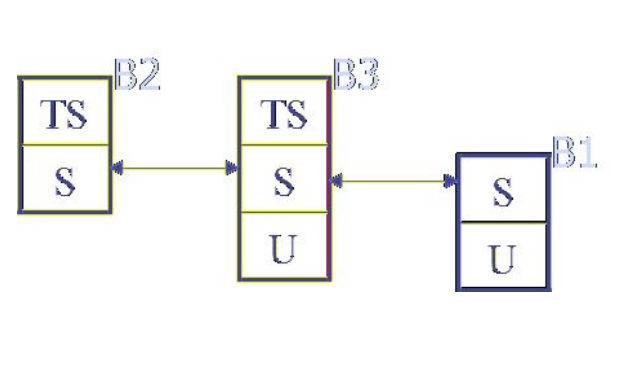
\includegraphics[width=8cm, keepaspectratio]{capitoli/policy/imgs/cascade1.png}
\end{figure}
I livelli di sicurezza delle macchine sono B1, B2 e B3. Lo
sforzo (l’effort) viene effettuato da un attaccante, il quale
cerca di penetrare una macchina con un determinato livello
di sicurezza.
Il “\textbf{cascade attack}” si ha quando una sola macchina viene attaccata ad 
un certo livello, ma anche
le altre vengono coinvolte conseguentemente.
L’informazione tra i sistemi è condivisa, quindi può fluire tra le macchine. 
Nell’esempio, infatti, sono
tutte collegate a livello S. Grazie all’effort su B2 si riesce a portare 
l'informazione da TS a U, che
equivale a dire di aver buttato giù un sistema B3. Quindi, a partire da B2, 
si riesce a buttar giù
anche B1 e B3.
Si dice “attacco a cascata” perché grazie ad uno sforzo relativamente piccolo 
(nel nostro caso
effettuato su B2) si possono attaccare anche sistemi più grandi e sicuri, 
poiché sono interconnessi.
In generale quindi, se l’attacco ha successo, il livello di segretezza può 
essere abbassato da
TopSecret a Secret, fino a Unclassified.
Si ha un “cascading attack” se esiste un “cascading path”, ovvero un cammino 
tra sistemi che
costa meno dello sforzo necessario a rompere i singoli sistemi.
Ricordiamo che eliminare i cascade path è un problema che rientra in NP.

\paragraph{Come eliminate il Cascade Path}
\begin{itemize}
      \item  Si possono disconnettere le macchine. Più c’è condivisione,
            più si alza la possibilità di
            avere cascading path;
      \item  Mettere in comunicazione le macchine a livelli diversi;
      \item  Definire i flussi consentiti (ognuno avrà uno specifico costo).
\end{itemize}
Il seguente non è un cascading path (non va bene perché dovremmo
rompere un sistema B3. L’effort è uguale all’attacco, non c’è il
guadagno).
\begin{figure}[H]
      \centering
      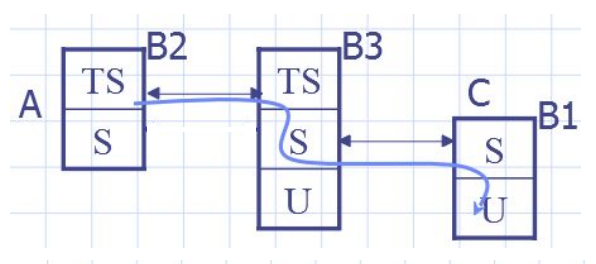
\includegraphics[width=8cm, keepaspectratio]{capitoli/policy/imgs/cascade3.png}
\end{figure}
Questo invece è un cascading path (quando il livello dell’attacco è più
grande dello sforzo).
\begin{figure}[H]
      \centering
      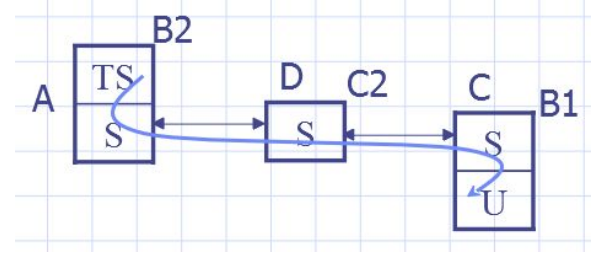
\includegraphics[width=8cm, keepaspectratio]{capitoli/policy/imgs/cascade2.png}
\end{figure}

\subsection{Secure Interoperation}